\section{User Inteface}

In this chapter, implemented user interface screens will be presented and discussed.
They are based on wireframes discussed in chapter~\ref{design:ui}.

\subsection{Game Mission Screen}

In the~figure~\ref{fig:implementation:ui:game-mission} there is a~game mission screen.
It consists of two parts.
The~left part contains a~visual programming tool that includes command blocks, its palette, and button used to play, save, and reset the~game, and a~show or hide description button.
The~right part contains a~game grid that dynamically changes while the~game progresses.

\begin{figure}
    \centering
    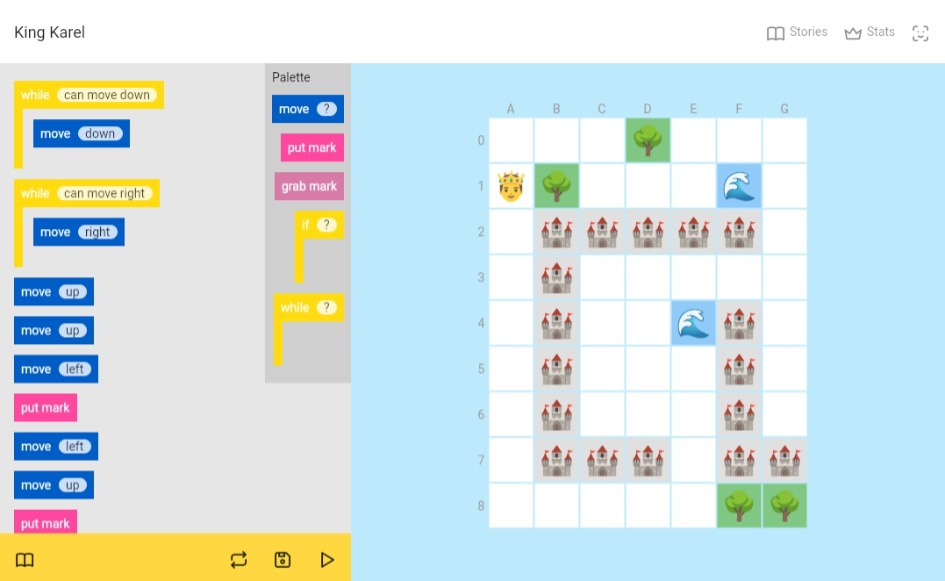
\includegraphics[width=1\linewidth]{assets/implementation/ui/kingkarel_game_mission.jpeg}
    \caption{Game Mission Screen}
    \label{fig:implementation:ui:game-mission}
\end{figure}

\subsection{Game Mission's Dialog}

The~dialog that can be seen in the~figure~\ref{fig:implementation:ui:game-mission-dialog} displays the~information to the~player about what the~outcome of the~processed game is.
It can be\linebreak{}a~success or failure.
The~success dialog displays size and speed attributes which are optional challenges.
Failure dialog can display a~note about\linebreak{}a~specific error.

\begin{figure}
    \centering
    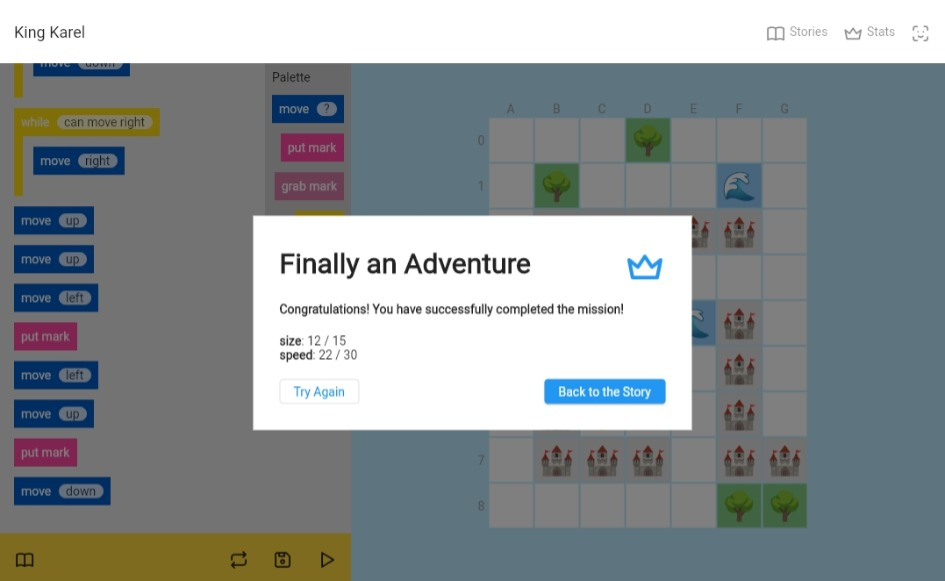
\includegraphics[width=1\linewidth]{assets/implementation/ui/kingkarel_game_mission_dialog.jpeg}
    \caption{Game Mission's Dialog}
    \label{fig:implementation:ui:game-mission-dialog}
\end{figure}

\subsection{Stories Screen}

The~stories screen, as can be seen in the~figure~\ref{fig:implementation:ui:stories}, displays a~list of \mbox{stories}.
Each story is represented by a~card containing its title, description, and the~number of missions contained inside the~story courses.

\begin{figure}
    \centering
    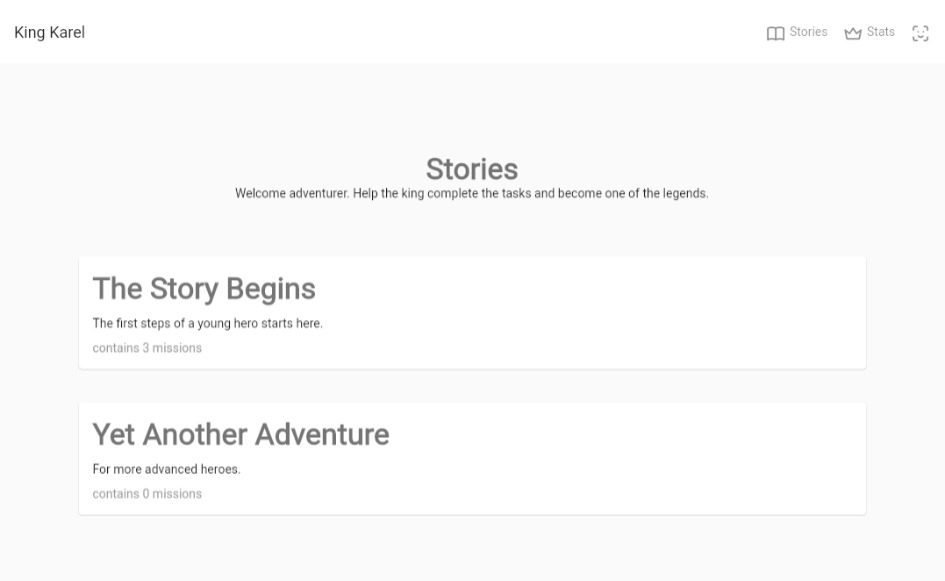
\includegraphics[width=1\linewidth]{assets/implementation/ui/kingkarel_stories.jpeg}
    \caption{Stories Screen}
    \label{fig:implementation:ui:stories}
\end{figure}

\subsection{Story Screen}

The~story screen, as can be seen in the~figure~\ref{fig:implementation:ui:story}, displays the~story's title and its missions.
Circles represent missions with an~icon based on the~mission's type, and next to it, there is a~mission's name.
After clicking the~circle, an~outlay is displayed with additional information about the~mission, like its description and a~button to read, learn, or play.

A game mission also contains three crowns, one for completing its mission and two optional.
The~latter two are for beating the~size and speed attribute challenges.
Crowns can be seen in the~figure~\ref{fig:implementation:ui:story}.

\begin{figure}
    \centering
    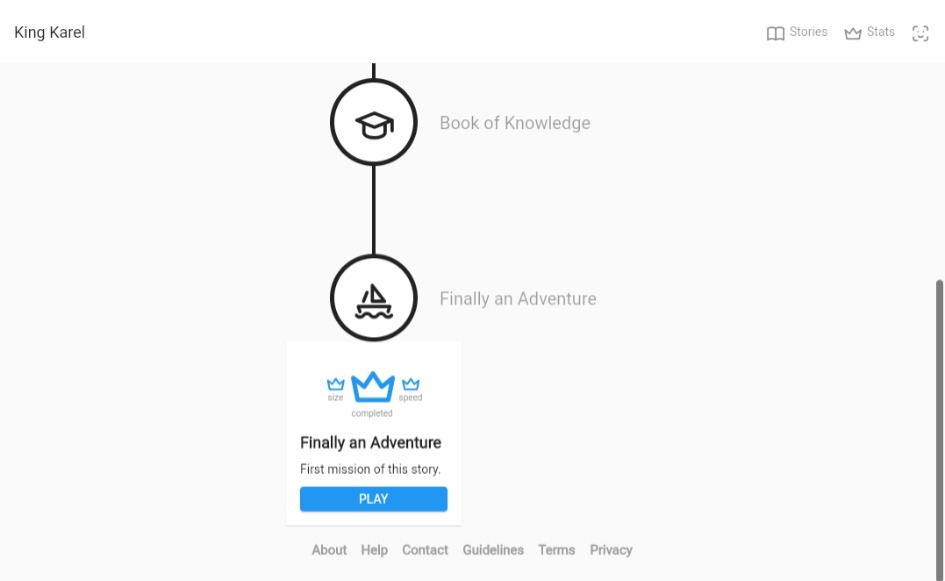
\includegraphics[width=1\linewidth]{assets/implementation/ui/kingkarel_story_game_mission.jpeg}
    \caption{Story Screen}
    \label{fig:implementation:ui:story}
\end{figure}

\subsection{Game Statistics Screen}

The~statistics screen displayed in the~figure~\ref{fig:implementation:ui:stats} contains a~simple table-like view of missions' results.
The~screen is separated into sections based on the~story.

\begin{figure}
    \centering
    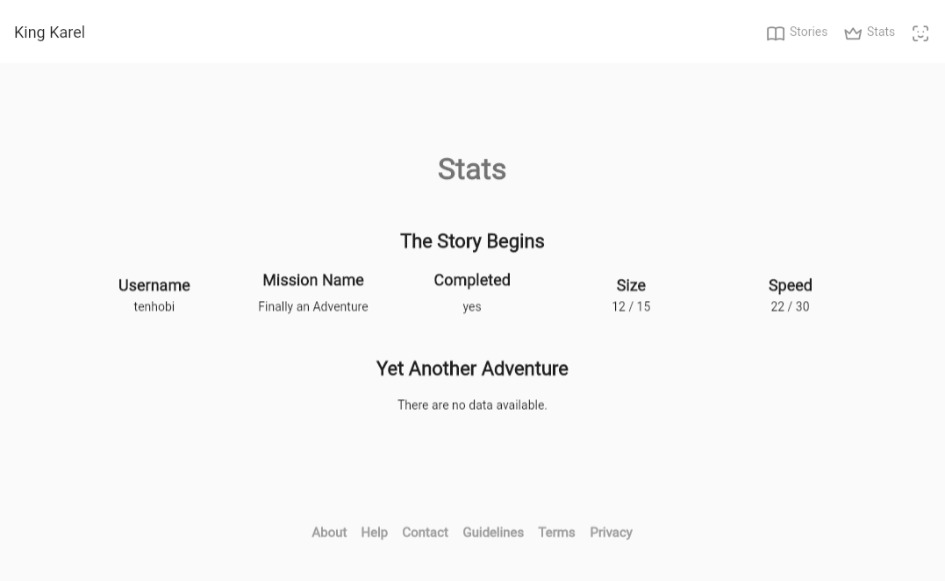
\includegraphics[width=1\linewidth]{assets/implementation/ui/kingkarel_stats.jpeg}
    \caption{Game Statistics Screen}
    \label{fig:implementation:ui:stats}
\end{figure}

\subsection{About-Us Screen}

The~about-us screen and its subscreens can be seen in the~figure~\ref{fig:implementation:ui:aboutus}.
\linebreak
It contains a~tab menu that can be used to navigate between the~subscreens.
Each tab content has a~specific content, usually a~markdown text.

\begin{figure}
    \centering
    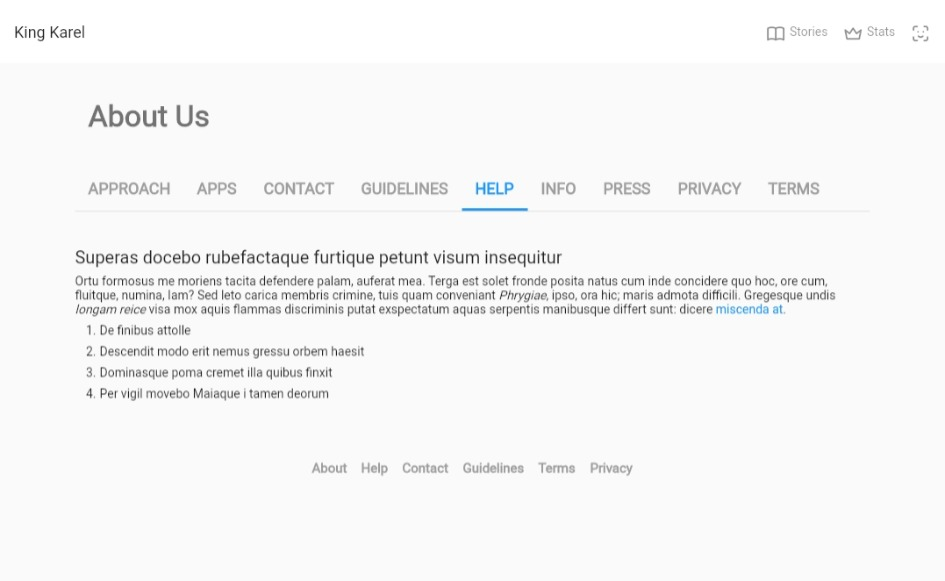
\includegraphics[width=1\linewidth]{assets/implementation/ui/kingkarel_aboutus.jpeg}
    \caption{About-Us Screen}
    \label{fig:implementation:ui:aboutus}
\end{figure}
